\documentclass[onecolumn, 12pt]{book}

\usepackage[latin1]{inputenc}   
\usepackage{amsmath}
\usepackage{algorithm}
\usepackage{algorithmic} 
%\usepackage[T1]{fontenc}

%\usepackage[francais]{babel}     
\usepackage{layout}    
\usepackage[top=2cm, bottom=2cm, left=2cm, right=2cm]{geometry} 
\usepackage{setspace}
\usepackage{soul}
\usepackage{color} 
\usepackage{verbatim}
\usepackage{moreverb}
\usepackage{listings}
\usepackage{url}
\usepackage{graphicx}
%\usepackage{epstopdf}
\usepackage[outdir=/home/willy/Documents/latexDoc/redaction/fusion_fichiers/images_fusionChapitres/]{epstopdf}
%\usepackage[outdir=./../../fusion_fichiers/images_fusionChapitres/]{epstopdf}
%\usepackage[outdir=./]{epstopdf}
\usepackage{caption}
\usepackage{setspace}
 
 
% \title{Mod\`ele de Donn\'ees}
% \author{Willy Ehounou}
 %\date{01/06/15}
\title{Chapitre6 : Simulations sur donn\'ees al\'eatoires}
\author{Wilfried Ehounou}
\date{\oldstylenums{\today}} 

\newtheorem{definition}{D\'efinition}
\newtheorem{theorem}{Theorem}
\newtheorem{property}{Propri\'et\'e}
\newtheorem{claim}[theorem]{Claim}
\newtheorem{proposition}[theorem]{Proposition}
\newtheorem{lemma}[theorem]{Lemma}
\newtheorem{corollary}[theorem]{Corollary}
\newtheorem{conjecture}[theorem]{Conjecture}
\newtheorem{observation}{Observation}
\newtheorem{example}{Exemple}
\newtheorem{remark}{Remark}

%---- path figures ----
\graphicspath{
{/home/willy/Documents/latexDoc/redaction/fusion_fichiers/images_fusionChapitres/}
}
 
\begin{document}
\maketitle
\tableofcontents

\chapter{Simulation des algorithmes sur des r\'eseaux th\'eoriques}
Dans ce chapitre, nous \'evaluons les performances des algorithmes propos\'es pr\'ecisement l'algorithme de correction. Nous proc\'ederons en deux \'etapes. 
La premi\`ere \'etape consistera  \`a g\'en\'erer des line-graphes dont nous ajouterons des erreurs dans leurs matrices d'adjacence. Le but de l'algorithme de correction sera de corriger les erreurs ajout\'ees \`a partir des cliques d\'ecouvertes par l'algorithme de couverture. 
La seconde \'etape consid\'erera les graphes n'ayant aucune line-couverture (graphes iourtes). Sur ces graphes iourtes, nous ferons  une \'etude comparative entre les distances line th\'eoriques (propri\'et\'e \ref{proprieteGrapheIourte}) et propos\'es par l'algorithme de correction pour caliber les param\`etres de l'algorithme de correction. \newline
%Apr\`es une description de notre protocole de simulation, nous definirons les methodes de correction et les fonctions de co\^ut et pr\'esenterons les param\^etres qui resolvent le probl\`eme Proxi-line.
Apr\`es la d\'efinition des m\'ethodes de correction, erreurs et seuil de corr\'elation, des fonctions de co\^uts de la suppression et de l'ajout des ar\^etes, nous d\'ecrirons la g\'en\'eration d'un graphe de corr\'elation c'est-\`a-dire un line-graphe dont on a ajout\'e/supprim\'e des ar\^etes et nous deduirons les valeurs de param\`etres qui r\'esolvent le probl\`eme Proxi-line. 

%###################################
%#              	objectifs et definitions				#
%###################################
\section{D\'efinitions et objectif}
Consid\'erons le graphe non orient\'e $G = (V,E)$ d'un r\'eseau de flots de matrice d'adjacence $matA$ et son line-graphe $L(G) = (E, A)$ avec $A$ l'ensemble des ar\^etes.
La matrice $matE$ est la matrice d'adjacence de $L(G)$ dont chaque case est not\'ee $\mu[i,j]$. Elle est aussi appel\'e matrice de corr\'elation binaire.
La matrice de corr\'elation $M$ de dimension $|E| \times |E|$ est form\'ee de cases $\mu_c[i,j]$ contenant des valeurs de corr\'elations comprise entre $0$ et $1$. 
Appliqu\'e une seuil de corr\'elation  $s$ \`a la matrice $M$, on obtient la matrice $matE$. On en d\'eduit que la matrice de corr\'elation de $L(G)$ est $M$. \newline
Le line-graphe $L(G)$, dont on ajoute des erreurs de corr\'elations (modification de cases $\mu$) dans sa matrice d'adjacence, est not\'e $G'$. Les matrice d'adjacence et de corr\'elation de $G'$ sont $matE'$ et $M'$ respectivement. Les cases des matrices $matE'$ et $M'$ sont not\'ees  $\mu'[i,j]$ et $\mu'_c[i,j]$ respectivement.
 
\subsection{D\'efinitions}

\begin{definition}
Une corr\'elation entre ar\^etes est l'existence d'un sommet commun aux ar\^etes. 
Ce sommet commun peut \^etre source, destination ou interm\'ediaire comme pr\'esent\'e dans la figure \ref{typeSommetEnCommun}.
\begin{figure}[htb!] 
\centering
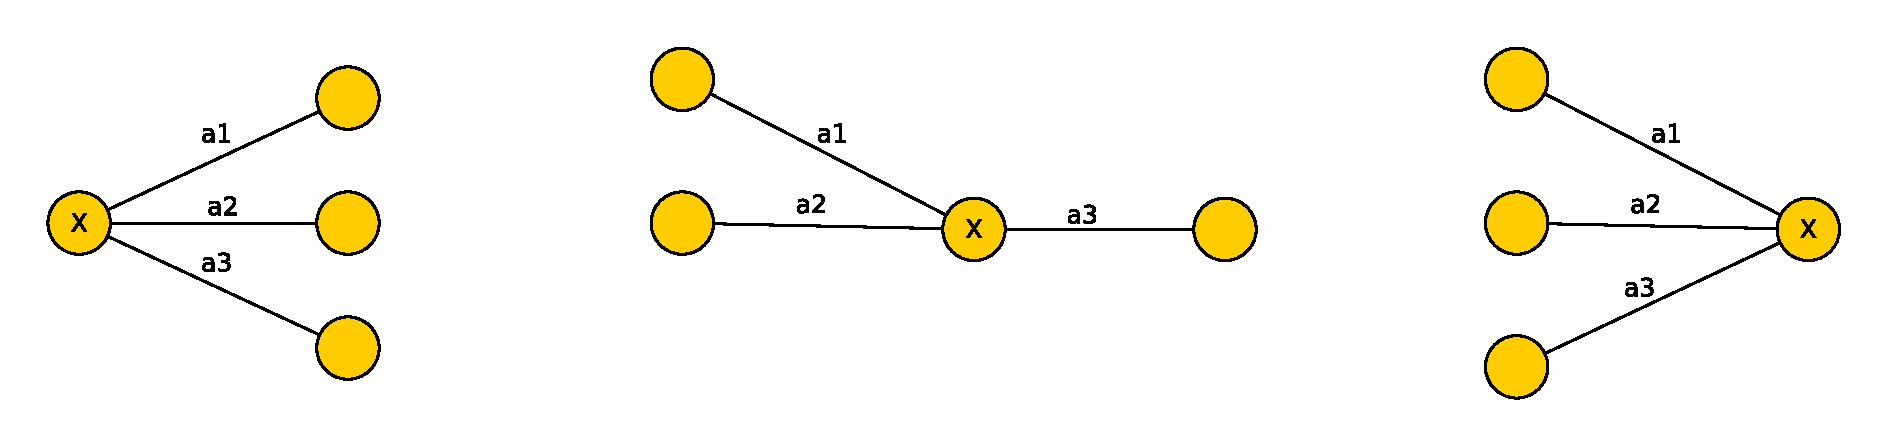
\includegraphics[scale=0.50]{typeSommetsEnCommun.eps}
\caption{De la gauche \`a la droite: sommet $X$ source, sommet $X$ interm\'ediaire, sommet $X$ destination}
\label{typeSommetEnCommun} 
\end{figure}
\end{definition}
Dans la matrice d'adjacence $matE$ de $L(G)$, une case \`a $\mu[i,j] = 1$ d\'esigne deux ar\^etes partageant un sommet dans $G$ alors que la case \`a $\mu[i,j] = 0$ implique que deux ar\^etes n'ont aucuns sommets en commun dans $G$. 
\newline
Par ailleurs, une case \`a $\mu[i,j] = 1$ signifie que sa valeur de corr\'elation  est comprise entre $s$ et $1$ ($s \le \mu_c[i,j] \le 1$) tandis que $\mu[i,j] = 0$ implique une valeur de corr\'elation comprise entre $0$ et $s$ ($0 \le \mu_c[i,j] < s$). 
Dans la r\'ealit\'e, nous avons des corr\'elations ($0 \le \mu_c[i,j] < s$)  entre des ar\^etes qui ont un sommet en commun et aussi des ar\^etes ne partageant aucuns sommets qui ont des corr\'elations  ($s \le \mu_c[i,j] \le 1$). Ces situations engendrent des {\em erreurs de corr\'elations} dans $matE$.

\begin{definition}
Une {\bf erreur de corr\'elation} est la modification de la valeur d'une case $\mu[i,j]$  de la matrice d'adjacence $matE$ de $L(G)$.
\end{definition}
On distingue quatre cat\'egories d'erreurs de corr\'elation, regroup\'ees dans le tableau \ref{categoriesErreursCorrelation}. Il s'agit des corr\'elations 
\begin{itemize}
\item {\bf vrai positives} : Il s'agit de cases $\mu' = 1$ dans $matE'$ n'ayant pas \'et\'e modifi\'ees dans la matrice $matE$.
\item {\bf vrai n\'egatives} :  Il s'agit de cases $\mu' = 0$ dans $matE'$ n'ayant pas \'et\'e modifi\'ees dans la matrice $matE$.
\item {\bf faux positives} : Il s'agit de cases $\mu' = 0$ dans $matE'$ modifi\'ees dans la matrice $matE$.
\item {\bf faux n\'egatives} : Il s'agit de cases $\mu' = 1$ dans $matE'$ modifi\'ees dans la matrice $matE$.
\end{itemize}
% La corr\'elation {\em fausse n\'egative} (l'absence de corr\'elation) est d\'esign\'ee par la valeur $0$ dans la matrice d'adjacence $matE'$ tandis que la corr\'elation {\em fausse positive} (l'existence de corr\'elation) a une valeur $1$ dans cette matrice. (voir tableau \ref{categoriesErreursCorrelation})
  La corr\'elation {\em fausse n\'egative} (l'absence de corr\'elation) est d\'esign\'ee par la valeur $0$ dans la matrice d'adjacence $matE'$ alors que sa case correspondante dans la matrice $matE$ a la valeur $1$. De m\^eme, dans  une corr\'elation {\em fausse positive} (l'existence de corr\'elation), la case  de valeur $1$ dans la matrice $matE'$ est transform\'ee en $0$ dans la matrice $matE$. (voir tableau \ref{categoriesErreursCorrelation}).
\begin{table}[h]
	\centering
	\begin{tabular}{ p{3em} p{3em} p{10em} }
		$L(G)$ & $L(G')$ & $\hspace{1 em}$ corr\'elations \\
		0 & 0 & $\rightarrow$ vrai n\'egative \\
		0 & 1 & $\rightarrow$ fausse positive \\
		1 & 0 & $\rightarrow$ fausse n\'egative \\
		1 & 1 & $\rightarrow$ vrai positive \\
	\end{tabular}
	\caption{ \label{categoriesErreursCorrelation}  Les types d'erreurs dans les matrices d'adjacence de $L(G)$ et $L(G')$}
\end{table}
\newline
% comment departager les erreurs de correlations? p_correl
% quel est la valeur de correlation pour chaque erreur de correlation
La distinction entre ces erreurs est faite par le seuil d'erreur de corr\'elation $p\_correl$.
\begin{definition} {seuil d'erreur de corr\'elation $p\_correl$} \newline
Le seuil d'erreur de corr\'elation est une valeur de corr\'elation partageant les erreurs de corr\'elations en deux sous-ensembles disjoints : faux n\'egatifs et faux positives. \newline
Si  $p\_correl \le \mu_c[i,j]< s$ $\rightarrow$ on a l'ensemble des corr\'elations fausses positives. \newline
Si $p\_correl - s \le \mu_c[i,j]< p\_correl$ $\rightarrow$  on a l'ensemble des corr\'elations fausses n\'egatives.
\end{definition}

\begin{figure}[htb!] 
\centering
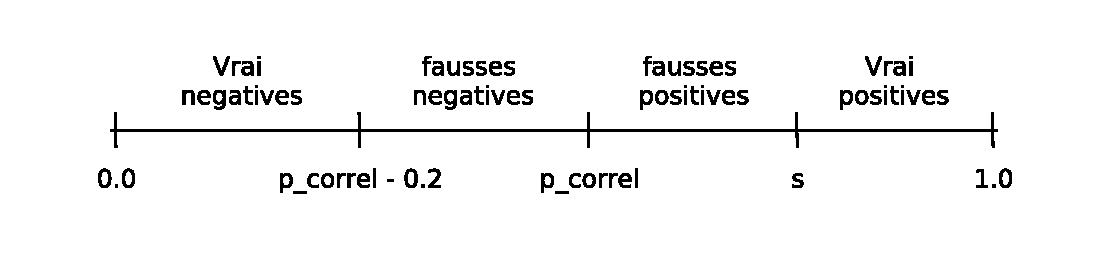
\includegraphics[scale=0.750]{intervallesFauxPositivesNegatives.eps}
\caption{ Correspondance entre valeurs et types de corr\'elations }
\label{intervallesFauxPositivesNegatives} 
\end{figure}

La figure \ref{intervallesFauxPositivesNegatives} r\'esume les valeurs de corr\'elations prises par chaque erreur. Ces valeurs sont regroup\'ees en quatre intervalles :
\begin{itemize}
\item {\em vrai n\'egatives} $\rightarrow$ $int\_vn = [0, p\_correl - s[$
\item {\em fausses n\'egatives} $\rightarrow$ $int\_fn = [p\_correl - s, p\_correl[$
\item {\em fausse positives} $\rightarrow$ $int\_fp = [p\_correl, s[$
\item {\em vrai positives} $\rightarrow$ $int\_vp = [s, 1]$
\end{itemize}
Dans le cas o\`u la matrice $matE$ ne contient aucunes erreurs de corr\'elations, alors $p\_correl = s$.

% graphe de correlation
\begin{definition}{ graphe de corr\'elation } \newline
Un graphe de corr\'elation $G'$ est un line-graphe dont on a introduit des erreurs de corr\'elation.
\end{definition}
G\'en\'eralement, le graphe de corr\'elation $G'$ n'est pas  un line-graphe. Toutefois, s'il est un line-graphe alors son graphe racine $L^{-1}(G')$ est diff\'erent du graphe $G$ ($G \neq L^{-1}(G')$).
% methode de correction
\begin{definition}{ m\'ethode de correction } \newline
Un m\'ethode de correction est l'ordre dans lequel on traite des sommets non couverts par aucune clique dans l'algorithme de correction.
\end{definition}

% fonction de cout
\begin{definition}{ fonction de co\^ut d'un sommet} \newline
La fonction de co\^ut d'un sommet est le co\^ut de chaque ar\^ete ajout\'ee ou supprim\'ee \`a son voisinage lorsqu'on applique l'algorithme de correction sur ce sommet.
\end{definition}

\subsection{Objectif}
Le but de cette \'etude est de montrer que nos algorithmes (couverture et correction) proposent
toujours un line-graphe connexe de distance de Hamming minimale 
\`a condition que la matrice du graphe de corr\'elation contienne $k<6$ d'erreurs de corr\'elations
et que les corr\'elations {\bf fausses n\'egatives} repr\'esentent plus de $65\%$ des erreurs de la matrice de corr\'elation.
En outre, nous montrerons la relation existance entre la distance line et celle de Hamming afin d'utiliser la distance line comme une m\'etrique dans les cas o\`u il est impossible de calculer la distance de Hamming (cas du graphe iourte).

%##########################################
%#               generation  graphes de correlation				  #
%# 			(protocole de simulation)					  #
%##########################################
\section{G\'en\'eration d'un graphe de corr\'elation}
Pour obtenir un graphe de corr\'elation $G'$, nous allons g\'en\'erer un r\'eseau de flots et   lui associer des mesures \'electriques sur chacune des ar\^etes. Ensuite, nous produirons la matrice de  corr\'elation binaire $matE$ li\'ee \`a ce r\'eseau. Enfin nous introduirons $k$ erreurs de corr\'elations dans la matrice $matE$.

\subsection{Construction d'un r\'eseau \'energ\'etique $G$}
Soient $n$ le nombre de sommets et $m$ le nombre d'ar\^etes.
On choisit $\alpha$ le degr\'e moyen de $G$.
\newline
On g\'en\`ere un graphe $G$ de $n$ sommets, de $m$ ar\^etes et dont la probabilit\'e d'existence d'une ar\^ete entre deux sommets est de $\frac{\alpha}{n}$. Si $G$ n'est pas connexe, nous choisissons al\'eatoirement un sommet de chaque composante connexe et nous ajoutons une ar\^ete entre ces sommets. 
\newline
Nous choisissons les sommets de degr\'e minimum comme des sources de notre tri topologique.
Nous effectuons ce tri avec un parcours en largeur {\em Breast First Search (BFS)} dans le graphe $G$.
Chaque sommet $x$ a un ordre topologique $D_x$ et l'ar\^ete $a_{xy}$ devient soit l'arc $a_{xy}$ si $D_x < D_y$ soit l'arc $a_{yx}$ si $D_x > D_y$. 
Le graphe obtenu est alors orient\'e (un {\em DAG} {\em Directed Acyclic Graph} ).
\newline
L'ajout des mesures depend du r\'eseau \'energ\'etique \`a mod\'eliser et des grandeurs physiques \`a observer. 
Dans le cas d'un r\'eseau \'electrique basse tension sinusoidal, nous choisirons l'intensit\'e ($I$), la tension ($U$) et la puissance ($P$) parce que certaines grandeurs physiques n'apportent aucune information (puissance r\'eactive constante ($Q$)) et certains param\`etres du r\'eseau sont inconnus (le facteur de puissance ($cos \phi$)).
L'intensit\'e varie entre $150A$ et $200A$, la tension entre  $220V$ et $250V$. 
En supposant que la r\'esistance des c\^ables \'electriques est n\'egligeable et que $cos \phi \approx 1$ , la puissance varie de $33000W$ et $62500W$ en s'inspirant de la formule $P = U \times I \times cos \phi$.
\newline
L'attribution des mesures pour chaque grandeur physique se fait \'egalement par parcours en largeur $(BFS)$. 
En effet,  on d\'ebute par les sommets sources et on g\'en\`ere une valeur al\'eatoire comprise dans l'intervalle de la grandeur physique. 
Chaque arc sortant du sommet source re\c coit  un flot \'egal \`a la somme des flots sur les arcs entrants du sommet source multipli\'ee par le facteur $\epsilon$ (d\'esignant les pertes par effets joules) et divis\'ee par le degr\'e sortant de ce sommet si nous avons comme grandeurs les intensit\'es et les puissances.
Dans le cas de grandeurs comme les tensions, le flot de chaque arc sortant est le flot multipli\'ee par le facteur $\epsilon$. 
On propage les valeurs de la grandeur physique jusqu'aux sommets puits (les \'equipements consommateurs d'\'energie).
L'application de ces r\`egles de flots permettent de v\'erifier la {\em loi de conversation des noeuds} \cite{loiDeConservation}.

\subsection{Construction de la matrice de corr\'elation}
\'Etant donn\'e que la corr\'elation entre ar\^etes est indiff\'erente \`a la position du sommet dans celles-ci, la matrice de corr\'elation binaire est la matrice $matE$ d'adjacence du line-graphe $L(G)= (E, A)$. %sous-jacent au graphe non orient\'e de $G$.
\newline
Nous consid\'erons la symm\'etrie sup\'erieure de $matE$ car $G=(V,E)$ est un graphe non orient\'e. 
Toutes les cases $\mu_G[i,j] = 1$ de $matA$ sont num\'erot\'ees sous la forme $(i,j)$ et forment les sommets de la matrice $matE$. Lorsque deux ar\^etes ont un sommet commun c'est-\`a-dire $\mu_G[i,j]  = \mu_G[j,k] $ ou $\mu_G[i,j]  = \mu_G[k,j]$ ou $\mu_G[j,i]  = \mu_G[k,j] $ alors la case de $matE$ re\c coit $1$ ($\mu[i',j'] = 1$ avec $i' = (i,j) \in A$ et $j' = (j,k) \in A$).
\newline
La matrice de correction $M$ contient des valeurs de corr\'elation probabilistes. 
Chaque case $\mu_c[i,j]$ de $M$ contient une corr\'elation calcul\'e selon  le type d'erreur associ\'e \`a celui-ci. 
Pour ce faire, nous consid\'erons deux cas :
\subsubsection{Cas 1 : $matE$ ne contient pas d'erreurs }
Dans ce cas, la variable de seuil de corr\'elation $p\_correl$ est le seuil $s$ ($p\_correl = s$). 
Nous allons g\'en\'erer les corr\'elations {\em vrai positives}  selon la loi exponentielle de param\`etre $\lambda \ge 2$ et les corr\'elations {\em vrai n\'egatives} selon la loi exponentielle de param\`etre $\lambda \ge -2$. Cela donne des distributions repr\'esent\'ees sur la figure \ref{vraiPositivesNegativesAutourDuSeuil}.
\subsubsection{Cas 2 : $matE$ contient d'erreurs }
Nous distinguons les quatres types d'erreurs de corr\'elations. Les corr\'elations {\em vrai positives} et {\em vrai n\'egatives}  suivent  la loi exponentielle de param\`etre $\lambda \ge 2$ et de param\`etre $\lambda \ge -2$ respectivement. 
Les corr\'elations {\em fausses positives et fausses n\'egatives} se localisent autour du seuil $p\_correl$ et  suivent des lois normales. La figure \ref{distributionErreursCorrelations} pr\'esente les courbes des distributions des  diff\'erentes erreurs de corr\'elation.
\begin{figure}[htb!] 
\centering
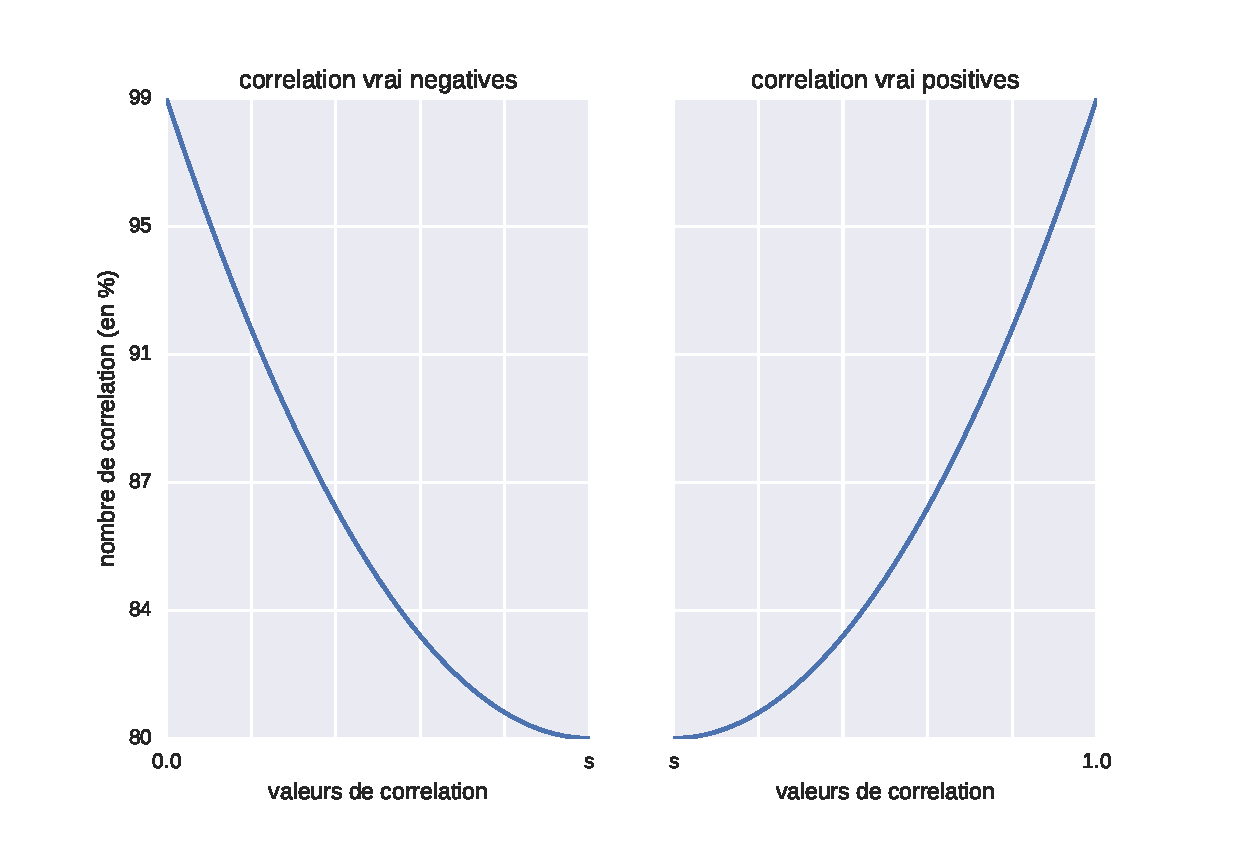
\includegraphics[scale=0.750]{vraiPositivesNegativesAutourDuSeuil.eps}
\caption{\`A gauche : Parabole croissante pour les erreurs {vrai positives} dans l'intervalle  $[s,1]$, \`a droite : Parabole d\'ecroissante pour les erreurs {vrai n\'egatives} dans l'intervalle $[0.s[$. L'ordonn\'e d\'esigne le taux de corr\'elation pour une valeur donn\'ee. }
\label{vraiPositivesNegativesAutourDuSeuil} 
\end{figure}

\begin{figure}[htb!] 
\centering
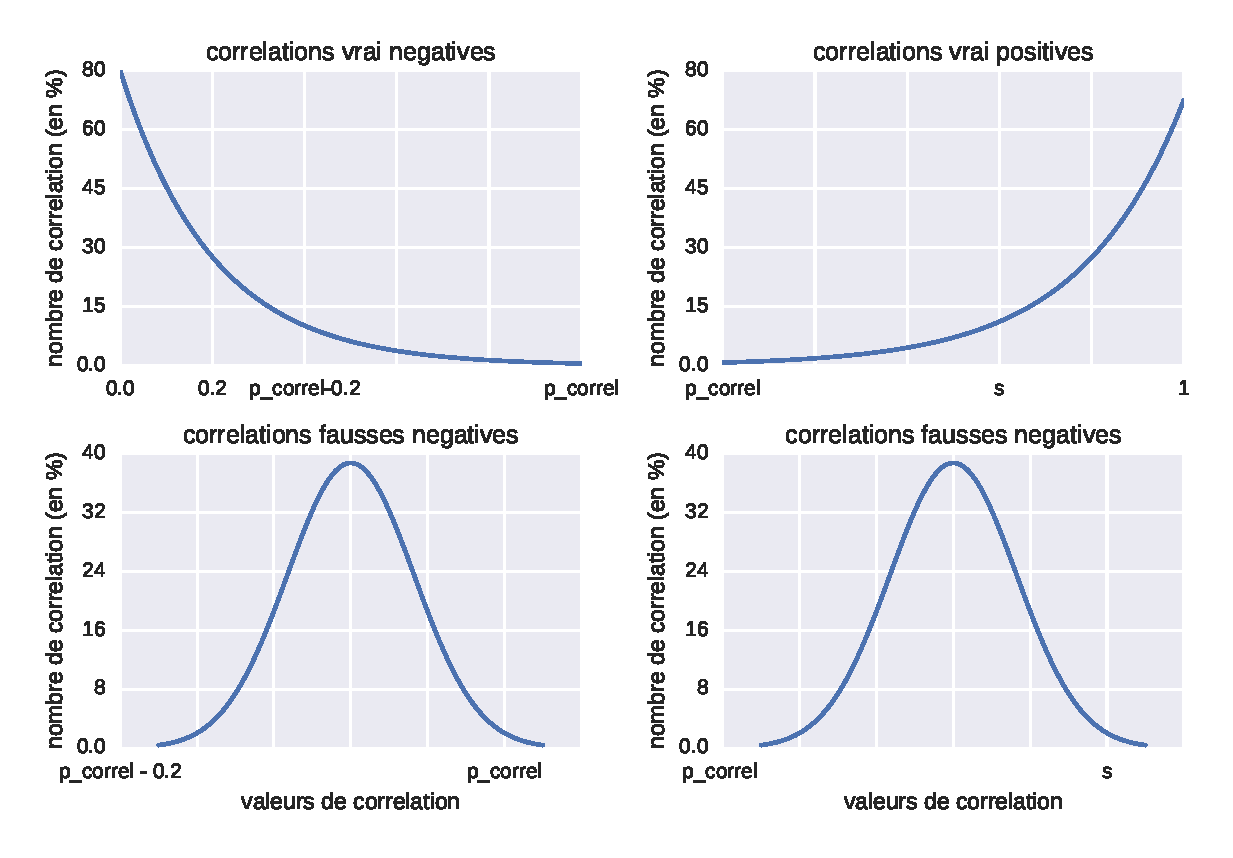
\includegraphics[scale=0.750]{distributionErreursCorrelations.eps}
\caption{En haut : loi exponentielle pour les erreurs   {\em vrai positives et vrai n\'egatives}, en bas : loi uniforme pour les erreurs   {\em fausses positives et fausses n\'egatives} }
\label{distributionErreursCorrelations} 
\end{figure}

 
L'utilisation de lois de probabilit\'e a pour but de montrer l'impact de seuil $p\_correl$ sur la line-couverture et aussi calculer les co\^uts de correction des sommets n'appartenant \`a aucune clique.

%##########################################
%#               correction graphes de correlation avec erreurs          #
%##########################################
\section{Correction d'un graphe de corr\'elation}


%#############################
%#               correction graphes iourtes           #
%#############################
\section{Correction des Graphes Iourtes}


%#############################
%#               conclusion				          #
%#############################
\section{Conclusion}

\end{document}